
\begin{frame}{‌روش درخت بازگشت}
\begin{itemize}\itemr
\item[-]
روش دیگر برای حل مسائل بازگشتی، استفاده از درخت بازگشت
\fn{1}{recursion tree}
است.
\item[-]
در این روش هر رأس از درخت، هزینه محاسبات یکی از زیر مسئله‌ها را نشان می‌دهد.
\item[-]
هزینهٔ کل اجرای یک برنامه عبارت است از هزینه‌ای که در سطح صفر درخت برای تقسیم و ترکیب نیاز است به علاوه هزینه محاسبه زیر مسئله‌ها. به همین ترتیب هزینه محاسبه هر یک از زیر مسئله‌های سطح اول تشکیل می‌شود از هزینه تقسیم و ترکیب به علاوهٔ هزینهٔ زیر مسئله‌های سطح دوم و به همین ترتیب الی آخر.
\item[-]
بنابراین اگر هزینهٔ محاسبهٔ همه رئوس درخت بازگشت را جمع کنیم، هزینه کل اجرای برنامه به دست می‌آید.
\end{itemize}
\end{frame}


\begin{frame}{‌روش درخت بازگشت}
\begin{itemize}\itemr
\item[-]
یک مثال درخت بازگشت را در اینجا بررسی می‌کنیم. رابطهٔ بازگشتی
\m{T(n) = 3T(n/4) + \ath{n^2}}
را در نظر بگیرید.
\end{itemize}
\end{frame}


\begin{frame}{‌روش درخت بازگشت}
\begin{itemize}\itemr
\item[-]
شکل زیر تشکیل درخت بازگشت را برای این رابطه بازگشتی در دو مرحله اول نشان می‌دهد.
\begin{figure}
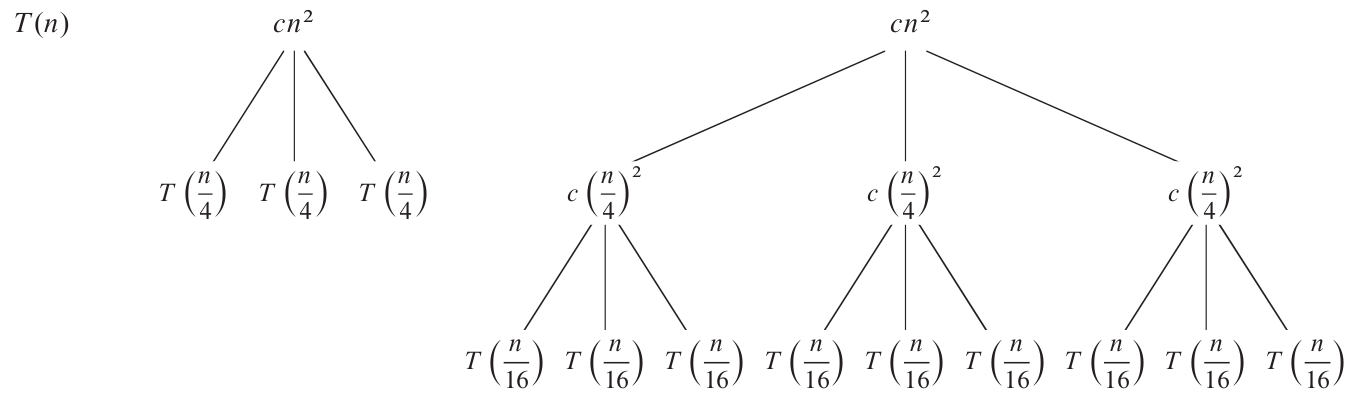
\includegraphics[width=1\textwidth]{figs/chap03/tree96-1}
\end{figure}
\end{itemize}
\end{frame}


\begin{frame}{‌روش درخت بازگشت}
\begin{itemize}\itemr
\item[-]
اگر مجموع هرینه‌ها را در هر سطح محاسبه کنیم، درختی با هزینه‌های قید شده در زیر خواهیم داشت.
\begin{figure}
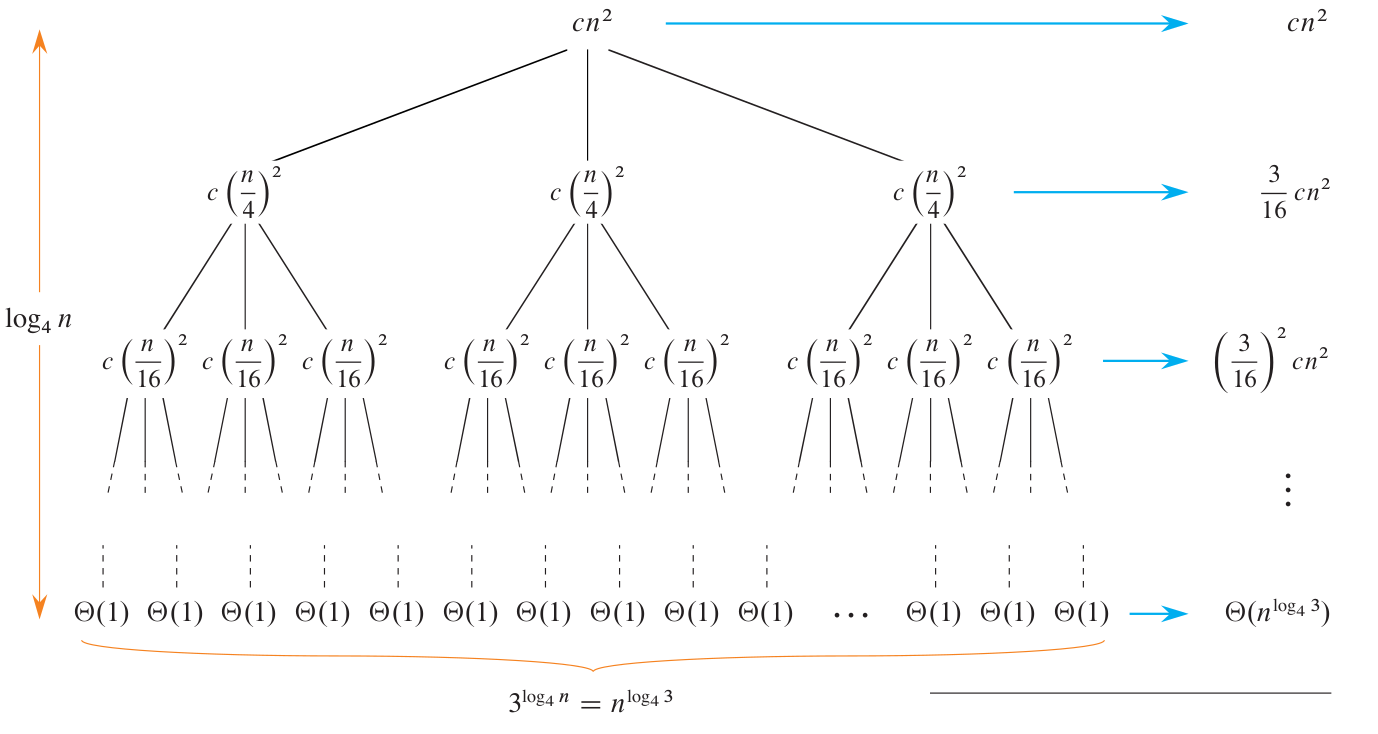
\includegraphics[width=0.9\textwidth]{figs/chap03/tree96-2}
\end{figure}
\end{itemize}
\end{frame}


\begin{frame}{‌روش درخت بازگشت}
\begin{itemize}\itemr
\item[-]
سپس هزینه‌های سطوح این درخت بازگشت را با هم جمع می‌کنیم و جواب رابطه بازگشتی را به دست می‌آوریم.
\end{itemize}
\end{frame}


\begin{frame}{‌روش درخت بازگشت}
\begin{itemize}\itemr
\item[-]
\begin{align*}
\m{T(n)} & \m{~= cn^2 + \frac{3}{16} cn^2 + {\left( \frac{3}{16} \right)}^2 cn^2 + \cdots +{\left( \frac{3}{16} \right)}^{\log_4 n} cn^2 + \ath {n^{\log_4 3}}}\\
& \m{~= {\sum_{i=0}^{\log_4 n}} {\left( \frac{3}{16} \right)}^i cn^2 + \ath {n^{\log_4 3}}} \\
& \m{~<  {\sum_{i=0}^{\infty}} {\left( \frac{3}{16} \right)}^i cn^2 + \ath {n^{\log_4 3}}}\\
& \m{~= \frac{1}{1 - (3/16)} cn^2 + \ath {n^{\log_4 3}}}\\
& \m{~= \frac{16}{13} cn^2 + \ath {n^{\log_4 3}}}\\
& \m{~= O(n^2)} ~~~~~~~~~~~~~~~~~~~~~~~~~~~~~~~~~~~ \m{(\ath {n^{\log_4 3}} = O(n^{0.8}) = O(n^2)).}
\end{align*}
\end{itemize}
\end{frame}
